
\section{Results}
The main results and findings go here.

Do not number an equation if it will not be directly cited in the
report. In order to avoid numbered equations, use
$\backslash$begin\{equation*\}--$\backslash$end\{equation*\},
$\backslash$[ --$\backslash$], or \$\$--\$\$.  For example:
\begin{equation*}
a = b + c,
\end{equation*}
$$\dot x = f(x,u) + g(x,u),$$
or
\[\ddot s=G(s,t)\]
where $f$, $g$, and $G$ are functions.

Note that Equation (\ref{equation-eqn1}) below is numbered!  It is
produced using $\backslash$begin\{equation\}--$\backslash$end\{equation\}:
\begin{equation}
F_i(P_i)=a_{i}+b_{i}P_i+c_{i}P_{i}^2
\label{equation-eqn1}
\end{equation}
where $a_{i},\ b_{i}$, and $c_{i}$ are coefficients of unit $i$, and $P_i$
represents some value for unit $i$.

Aligning equations can be done with
either the align or eqnarray commands.  Recently,
$\backslash$begin\{align\}--$\backslash$end\{align\} has gained popularity
over $\backslash$begin\{eqnarray\}--$\backslash$end\{eqnarray\}.

Equation (\ref{equation-eqn2}) is produced using
$\backslash$begin\{align\}--$\backslash$end\{align\}:
\begin{align}
\dot {x}_l=& \sum_{i = 1}^m {\frac{c_{P_{x_i} } e^{k_{x_i}\bar{x}_i} + c_{N_{x_i} }
e^{ -  k_{x_i} \bar{x}_i}}{e^{k_{x_i} \bar{x}_i} + e^{ - k_{x_i} \bar{x}_i}}} \nonumber\\
& + \frac{1}{2}\sum\limits_j^q (c_{P{u_j }} + c_{N _{u_j }} ) \nonumber\\
y=& \ A_0 + A_1 \tanh (K_x \bar {x}) + B\tanh (K_u \bar {u}) \nonumber\\
 =& \ F(x),
\label{equation-eqn2}
\end{align}
where $F(x)$ is a function.

Equation (\ref{equation-eqn3}) represents the same equation produced
using $\backslash$begin\{eqnarray\}--$\backslash$end\{eqnarray\}:
\begin{eqnarray}
\dot {x}_l&=& \sum_{i = 1}^m {\frac{c_{P_{x_i} } e^{k_{x_i}\bar{x}_i} + c_{N_{x_i} }
e^{ - k_{x_i} \bar{x}_i}}{e^{k_{x_i} \bar{x}_i} + e^{ - k_{x_i} \bar{x}_i}}} \nonumber\\
&&+ \frac{1}{2}\sum\limits_j^q (c_{P{u_j }} + c_{N _{u_j }} ) \nonumber\\
y&=& \ A_0 + A_1 \tanh (K_x \bar {x}) + B\tanh (K_u \bar {u})\nonumber\\
&=& \ F(x),
\label{equation-eqn3}
\end{eqnarray}
where $F(x)$ is a function.  You get the idea!

\subsection{Example of a Figure}
Below is an example of a floating figure using the graphicx
package.  Note that $\backslash$label must occur AFTER (or within)
$\backslash$caption.  For figures, $\backslash$caption should occur
after the $\backslash$includegraphics.  To reference a figure, use
the word Figure followed by the figure number.  Here is an example:
Figure~\ref{figure-fig1}.

\begin{figure}[htp]
\centerline{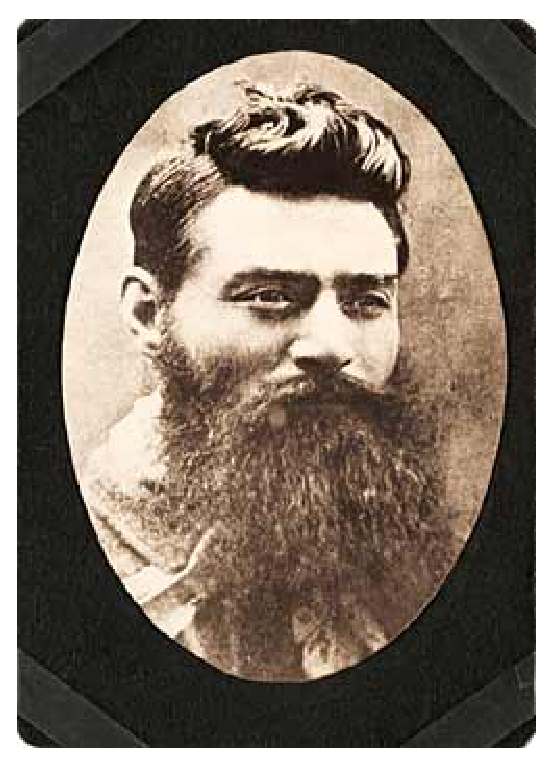
\includegraphics[width=0.6\columnwidth]{NedKelly.eps}}
\caption{A famous Australian bush-ranger: Ned Kelly}
\label{figure-fig1}
\end{figure}

\subsection{Figures and Tables}
Please follow the style in this sample paper when generating your figures
and tables.

\subsection{Page Limit and Overlength Page Charges}
A paper submitted to this conference should be prepared in a
single-spaced, two-column format.  Its length must be kept to 8
pages or less.  In exceptional circumstances, up to two additional
pages will be permitted for a charge of AUD\$100 per additional page.
Table~\ref{table-tab1} shows the page limit and page charge schedule.

% An example of a floating table.  Note that, the
% \caption command should come BEFORE the table.  Table text will default
% to \footnotesize.
% The \label must come after \caption as always.
\begin{table}
\begin{center}
%% Increase table row spacing; adjust to taste
\renewcommand{\arraystretch}{1.3}
\caption{Page Limit}
\label{table-tab1}
% The array package and the MDW tools package offers better commands
% for making tables than plain LaTeX2e's tabular which is used here.
\begin{tabular}{|c|c|}
\hline
Page limit: & 8\\
\hline
Excess page charge: & AUD\$100/page\\
\hline
\end{tabular}
\end{center}
\end{table}

Another example of a table is shown in Table~\ref{table-tab2}.

\begin{table}[h]
\caption{A second table}
\begin{center}
\begin{tabular}{|c|c|c|c|c|c|}
\hline
\multicolumn{1}{|c|}{\raisebox{-1.50ex}[0cm][0cm]{\!Method\!}}
& \multicolumn{1}{|c|}{Mean}
& \multicolumn{1}{|c|}{Best}
& \multicolumn{1}{|c|}{Mean}
& \multicolumn{1}{|c|}{Maximum}
& \multicolumn{1}{|c|}{Minimum} \\
& time & time & cost & cost & cost\\ \hline
A      &  $928.36$  &  $926.20$  &  $124793.5$ & $126902.9$ & $123488.3$ \\ \hline
B      &  $646.16$  &  $644.28$  &  $124119.4$ & $127245.9$ & $122679.7$ \\ \hline
C      &  $1056.8$  &  $1054.2$  &  $123489.7$ & $124356.5$ & $122647.6$ \\ \hline
D      &  $632.67$  &  $630.36$  &  $123382.0$ & $125740.6$ & $122624.4$ \\ \hline
\end{tabular}
\label{table-tab2}
\end{center}
\end{table}

Citations are included like so~\cite{book}.
Multiple citations appear like this~\cite{conf,article}.
